\documentclass[a4paper,12pt]{article}

\oddsidemargin=-4mm
\evensidemargin=-4mm
\textheight=255mm
\topmargin=-15mm
\textwidth=170mm
\headsep=10mm

\usepackage{amssymb,amsmath,amsfonts}
\usepackage[T2A]{fontenc}
\usepackage[english,russian]{babel}
\usepackage{graphicx}
\usepackage{epstopdf}

\let\chapter\section
\sloppy

\begin{document}

%%%%%%%%%%%%%%%%%%%%%%%%%%%%%%%%%%%%%%%%%%%%%%%%%%%%%%%%%%%%%%%%%%%%%%%%%%%%%%%%%%
\noindent
УДК: 532.546

{\large
\begin{center}
\textbf{О процессе выпадения парафина в пласте}\\
И.С.~Лазарев$^1$, А.И.~Никифоров$^2$
\end{center}
} 

{\footnotesize
\noindent $^1$ Lazarevigor.2001@mail.ru; КФУ, ИММ, им. Н.И.~Лобачевского \\
\noindent $^2$ nikiforov@imm.knc.ru; ФИЦ КазНЦ РАН, ИММ
}


\begin{abstract}
	В работе рассматривается задача двухфазной неизотермической фильтрации воды и нефти. Нефть моделируется как смесь двух несмешивающихся с водой углеводородных составляющих "нефти" и "парафина". Задача численно решается методом контрольных объемов. Для прогнозирования кристаллизации парафина применяется теория идеального раствора бинарной смеси. Основное внимание уделяется процессам осаждения частиц в пористой среде. Для уравнений, определяющих динамику изменения пористости и проницаемости, используются зависимости, основанные на функции распределения пор по размерам. 
\end{abstract}

\noindent
\textit{Ключевые слова:} парафиновые отложения, фильтрация, дисперсные частицы, кольматация, пористость, проницаемость, повреждение пласта.

%%%%%%%%%%%%%%%%%%%%%%%%%%%%%%%%%%%%%%%%%%%%%%%%%%%%%%%%%%%%%%%%%%%%%%%%%%%%%%%%%%

\vspace{1em}
\hrule

%%%%%%%%%%%%%%%%%%%%%%%%%%%%%%%%%%%%%%%%%%%%%%%%%%%%%%%%%%%%%%%%%%%%%%%%%%%%%%%%%%
\vspace{1em}
{\subsection*{\normalsize Введение}}
	В процессе разработки нефтегазовых месторождений температурные изменения, вызванные технологическими воздействиями, могут существенно влиять на физико-химические свойства пластовых флюидов. Особенно актуальной проблемой становится выделение парафина из нефти. Парафин выпадает в осадок, образуя дисперсные частицы, оседающие на поверхности пор. Это приводит к ухудшению фильтрационно-емкостных характеристик коллектора. В частности, кольматация пор парафином уменьшает пористость и проницаемость, а также увеличивает скин-фактора, что снижает продуктивность скважин. На это указывают многие исследования, связанные с анализом керна методом компьютерной томографии \cite{bib:01}. Таким образом, учет тепловых и химических факторов является неотъемлемой частью проектирования разработки месторождений.

\vspace{2em}
{\subsection*{\normalsize Законы сохранения}}
	В рассматриваемой модели присутствуют две фазы и три псевдокомпонента. Нефть и вода представляют собой две отдельные не смешивающиеся фазы. В качестве трех псевдокомпонентов выступают нефть, вода и парафин. Предполагается, что жидкости несжимаемы, а также что между водной и нефтяной фазами не происходит массообмен. Поэтому уравнения баланса масс записываются для каждой фазы отдельно. Учитывая сделанные допущения, уравнения баланса массы для воды и нефти, имеют следующую структуру:

\begin{equation}\label{eq1}
\frac{\partial }{\partial t}(m \rho_w S_w ) + \nabla(\rho_w \mathbf{U_w}) = q_w \rho_w,
\end{equation}

\begin{equation}\label{eq2}
\frac{\partial }{\partial t}(w_o  m \rho_o S_o) + \nabla(w_o \rho_o \mathbf{U_o}) = w_o q_o \rho_o.
\end{equation}

	Псевдокомпонент парафина может быть частично растворен и/или взвешен в нефтяной фазе в виде частиц и отложен в поровом пространстве. Уравнение баланса массы парафина в этом случае запишется в виде \cite{bib:02}:

\begin{equation}\label{eq3}
\frac{\partial}{\partial t}(w_{ps} m \rho_p S_o + w_p  m \rho_o S_o) + \nabla(w_{ps}  \rho_p \mathbf{U_o} + w_p \rho_o \mathbf{U_o}) = q_p \rho_p + q_o (w_p \rho_o + w_{ps} \rho_p).
\end{equation}

	Уравнения движения фаз представим с помощью закона Дарси в пренебрежении влиянием капиллярных и гравитационных сил:
\begin{equation}\label{eq4}
\mathbf{U_i} = \frac{k f_i}{\mu_i} \nabla P,  \qquad (i=o,w).
\end{equation}

	В рамках однотемпературной термодинамической модели  уравнение, описывающее баланс полной энергии всей системы, может быть сформулировано в виде следующего выражения \cite{bib:03}:

\begin{multline}\label{eq5}
\frac{\partial }
{\partial t}(m \rho_w S_w C_w T +(1-w_{ps})m \rho_o S_o C_o T + 
w_{ps}m \rho_p S_o C_p T +(1-m) \rho_f C_f T) + 
\\
+\nabla(\rho_w \mathbf{U_w} C_w T + (1-w_{ps}) \rho_o \mathbf{U_o} C_o T + w_{ps}\rho_p \mathbf{U_o} C_p T) = 
\\
=\nabla [(m S_w K_w + (1-w_{ps}) m S_o K_o  + w_{ps} m S_o K_p + (1-m) K_f) \nabla T ] + q_o \rho_o C_o T + q_w \rho_w C_w T
\end{multline}

Растворимость и осаждение парафинов из нефти моделируется уравнением теории идеального раствора для бинарной смеси \cite{bib:03}:
\begin{equation} \label{eq6}
w_{ps} = w_p \exp[\frac{\alpha}{R}(\frac{1}{T} - \frac{1}{T_m})]. 
\end{equation}

\vspace{1em}
{\subsection*{\normalsize Модель пористой среды}}
	 При описании кольматации пласта частицами парафина, будем рассматривать пористую среду в рамках модели идеального грунта, то есть как систему цилиндрических капилляров разного диаметра, имеющих фиктивные сужения (горла). Для простоты используем следующие допущения:
\begin{enumerate} 
	\item Для всех капилляров отношение радиуса горла к радиусу канала $\gamma :(0< \gamma \leq 1)$ одинаково и сохраняется в процессе кольматации частиц;
	\item Частицы парафина имеют шарообразную форму одинакового размера – диаметр $l$;
	\item Количество оседающих частиц пропорционально их долям в движущейся фазе;
	\item Капилляр полностью блокируется при попадании частиц, если характерный размер частиц не меньше диаметра горловины, равного по величине $\gamma r$;
	\item Собственная пористость осевших частиц пренебрежимо мала по сравнению с пористостью пласта;
	\item Суффозией пренебрегаем, ввиду сложности механизма взаимодействия частиц парафина и недостатка экспериментальных данных;
	\item Доля капилляров, занятых некоторой фазой, пропорциональна насыщенности образца этой фазой.
\end{enumerate}
Последнее допущение является отражением основной гипотезы модели двухфазной фильтрации. Согласно ей вода и нефть движутся по своим системам пор \cite{bib:05}.

\vspace{1em}
{\subsection*{\normalsize Структурные изменения пористой среды}}
	\textbf{Скорость сужения порового канала}. Исходя из экспериментальных данных была получена эмпирическая зависимость для скорости сужения цилиндрического порового канала в однофазном потоке, вызванная кольматацией \cite{bib:04}. По аналогии с однофазным потоком для двухфазного скорость сужения порового канала в случае оседания частиц парафина в нефти запишется в виде:
\begin{equation}\label{eq7}
\upsilon_r = -w_{ps} (S_o-S_{0}^{*}) \left ( \frac{2 \upsilon_{mo} D^2}{r L_k} \right )^{\frac{1}{3}}.
\end{equation}

\par \textbf{Скорость блокирования пор}. Для поровых каналов, занятых нефтью, размеры которых удовлетворяют условию блокирования $r \leq \frac{l}{2 \gamma}$, будем вычислять скорость блокирования по следующей формуле \cite{bib:04}:
	
\begin{equation}\label{eq8}
\upsilon_b = \left\{\begin{matrix}
\frac{(S_0-S_{o}^{*}) 6 \beta r^2 w_{ps} \upsilon_{mo} \phi}{l^3}, \quad \qquad r \leq \frac{l}{2 \gamma}
 \\
 0, \qquad \qquad \qquad \qquad \qquad r > \frac{l}{2 \gamma}
\end{matrix}\right.
\end{equation}

\par \textbf{Функция пор по размерам}. Для описания радиусов капилляров вводится функция пор по размерам, согласно которой $ \phi (r,t)-$ доля капилляров, имеющих радиус r в момент времени t. Будем полагать, что для начального момента времени (t = 0) функция пор по размерам известна т.е. $ \phi (r,0)= \phi_0 (r)$.
Кинематика изменения функции распределения пор по размерам во времени будет определяться следующим уравнением \cite{bib:05}:
\begin{equation}\label{eq9}
\frac{\partial \phi}{\partial t} + \frac{\partial (\upsilon_r \phi)}{\partial r} + \upsilon_b = 0.
\end{equation}
Подчеркнем, что изменение радиусов происходит во всех поровых каналах, а блокирование происходит только при размере частиц менее радиусов горловин поровых каналов. Однако могут блокироваться и каналы, для которых в начальный момент времени $r \geq \frac{l}{2 \gamma}$, так как в процессе кольматации пласта частицами парафина их диаметры уменьшились и стали удовлетворять условию закупоривания.

\par \textbf{Пористость и проницаемость}. В следствии структурных изменений порового пространства, вызванное кольматацией и блокированием пор, происходит изменение динамической пористости и абсолютной проницаемости пласта. Пусть $m_0$ и $k_0$ начальные пористость и проницаемость, тогда для текущего момента времени их можно представить в виде произведений: $m=m_f m_0$ и $k=k_f k_0$ соответственно. Фактор пористости $m_f$ определим, используя просветность \cite{bib:04}: 
\begin{equation}\label{eq10}
m_f = \frac
{ \int_{0}^{\infty} r^2 \phi (r) dr}
{ \int_{0}^{\infty} r^2 \phi_0 (r) dr}.
\end{equation}
Коэффициент $k_f$ определим, воспользовавшись моделью параллельных капилляров и законом Пуазейля \cite{bib:04}:

\begin{equation}\label{eq11}
k_f = \frac
{ \int_{0}^{\infty} r^4 \phi (r) dr}
{ \int_{0}^{\infty} r^4 \phi_0 (r) dr}.
\end{equation}

\par \textbf{Интенсивность массообмена}. Изменение объема взвешенных частиц парафина в нефти вызвано двумя факторами: оседание на поверхности пор и блокировка поровых нефтяных каналов \cite{bib:03}. Ввиду вышеуказанных допущений, скорость массообмена парафина в пористой среде будет равна:
\begin{equation}\label{eq12}
q_p =
2 m \frac{ \int_{0}^{\infty} r \upsilon_r(r) \phi (r) dr}{ \int_{0}^{\infty} r^2 \phi(r) dr} + 
w_{ps} m  \frac{ \int_{0}^{\infty} r \upsilon_b(r) \phi (r) dr}{ \int_{0}^{\infty} r^2 \phi(r) dr}.
\end{equation}


\vspace{1em}
{\subsection*{\normalsize Метод решения}}
	В качестве метода дискретизации дифференциальных уравнений (\ref{eq1})--(\ref{eq5}) использовался метод контрольных объемов. Согласно которому, при интегрировании уравнений предполагается, что характеристики пласта и флюидов на контрольном объеме имеют постоянные значения. Интегрирование конвективных слагаемых выполнялось по схеме вверх по потоку. А для совместного решения уравнений давления и насыщенности был использован метод IMPES (Implicit Pressure Explicit Saturation). Уравнение изменения функции пор по размерам (\ref{eq9}) решалось по неявной схеме. Это позволило избежать ограничений на шаг по времени в задаче расчета кольматации пласта парафином.

\vspace{1em}
{\subsection*{\normalsize Результаты}}
	Рассматривается двухфазная неизотермическая многокомпонентная фильтрация в прямоугольной области $D = [0, 200] \times [0, 200] \times [0, 1]$. Пласт является однородным, его пористость и проницаемость равны $m_0=0.2$  и $k_0=200$ мД соответственно. Область $D$ является элементом симметрии пятиточечной системы заводнения и содержит две вертикальные совершенные по степени вскрытия скважины радиуса $r_w = 0.1$ м. (нагнетательную и добывающую), имеющие координаты $(0,0)$ и $(200,200)$ соответственно. Начальная температура пласта $70^{\circ}$, а температура нагнетаемой воды $25^{\circ}$.
	\par Для анализа влияния растворенного парафина на процесс добычи нефти с закачкой холодной воды рассмотрим два случая: в первом происходит фильтрация парафиносодержащей многокомпонентной нефти $(W_p=5 \%)$ (черная сплошная линия), а во второй – обычная однокомпонентная нефть $(W_p=0 \%)$ (красная пунктирная линия). Расчет проводился до времени, когда обводненность добывающей скважины будет равна $98 \%$. В первом случае конечное время составило 2100.46 сут. и КИН=0.5098, а во втором - конечное время 1835.33 сут. и КИН=0.51375. Более долгий период времени достижения предельной обводненности добывающей скважины указывает на то, что кольматация парафина в поровом пространстве снижает скорость фильтрации. А сниженное значение КИН первой постановки по сравнению со второй говорит о том, что частицы парафина полностью заблокировали некоторые каналы, по которым продвигалась нефть. На графике (рис.~\ref{fig:01}) представлены дебеты воды и нефти добывающей скважины. Видно, что в случае кольматации пласта парафинам дебеты снизились, наиболее ярко выражено на графике дебета воды. В случае отсутствия растворенного парафина в момент времени $t\approx 1200$ суток дебет начал снижаться. Это вызвано тем, что в этот момент фронт низкой температуры достиг добывающей скважины, что привело к повышению вязкости флюидов, а впоследствии снижению продуктивности скважины. В случае наличия растворенного парафина в момент времени $t\approx 1600$ суток фронт воды также достиг добывающей скважины, но помимо увеличения вязкости флюидов дополнительно вызвал снижение фильтрационно-емкостных свойств пласта вблизи добывающей скважины. Поэтому в данном случае наблюдается более сильное падение дебета. На (рис.~\ref{fig:02}) изображены графики накопленной добычи нефти и воды. Заметно, что выпадение парафина сильно снизило объем закачиваемой воды. Это, в свою очередь, привело к падению пластового давления. Таким образом, низкая температура воды снизила эффективность закачки.

\vspace{1em}
{\subsection*{\normalsize Заключение}}
	Разработаная математическая модель (\ref{eq1})--(\ref{eq12}) позволяет моделировать изменения фильтрационно-емкостных свойств пористой среды на основе функции пор по размерам. А также прогнозировать, как данные изменения повлияют на нефтеотдачу в зависимости от конкретных геофизических условий и условий заводнения. Дальнейшее развитие модели возможно путем совершенствования термодинамической модели осаждения парафинов в нефтяных смесях.

\begin{figure}[h]
\begin{minipage}[h]{0.49\linewidth}
\centering
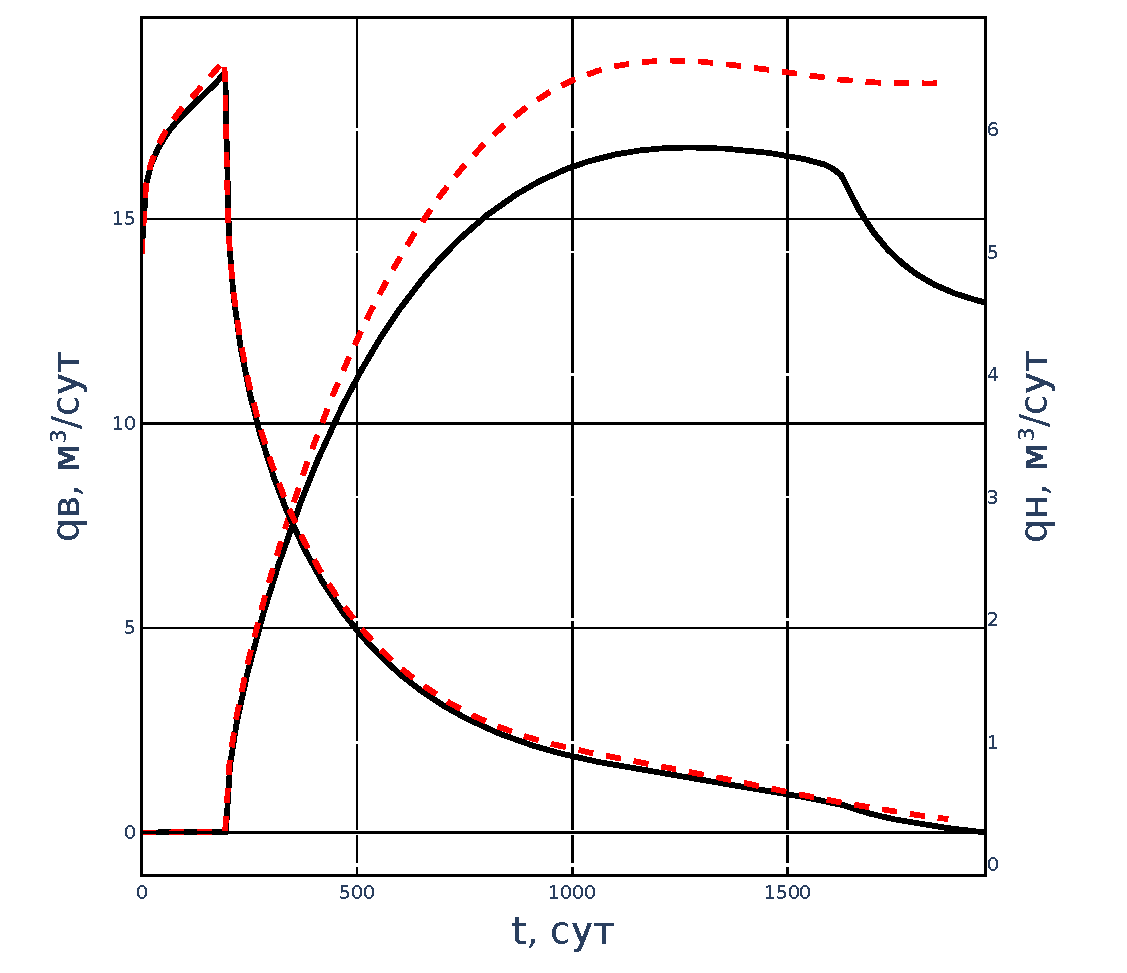
\includegraphics[width=0.85\linewidth]{LazarevIS_1.eps}
\caption{Дебеты воды и нефти добывающей скважины} 
\label{fig:01}
\end{minipage}
\hfill
\begin{minipage}[h]{0.49\linewidth}
\centering
\includegraphics[width=0.85\linewidth]{LazarevIS_2.eps}
\caption{Накопленные дебеты воды и нефти добывающей скважины} 
\label{fig:02}
\end{minipage}
\end{figure} 

%%%%%%%%%%%%%%%%%%%%%%%%%%%%%%%%%%%%%%%%%%%%%%%%%%%%%%%%%%%%%%%%%%%%%%%%%%%%

\bibliographystyle{gost2008}     
\bibliography{LazarevIS}   

%%%%%%%%%%%%%%%%%%%%%%%%%%%%%%%%%%%%%%%%%%%%%%%%%%%%%%%%%%%%%%%%%%%%%%%%%%%%%%%%

\begin{otherlanguage}{english}

{\large
\begin{center}
\textbf{About the process of paraffin deposition in the formation}\\
I.S.~Lazarev, A.I.~Nikiforov
\end{center}
}

\begin{abstract}
	This paper considers the problem of two-phase non-isothermal filtration of water and oil. Oil is modeled as a mixture of two immiscible hydrocarbon components, "oil" and "paraffin". The problem is solved numerically using the control volume method. The theory of an ideal binary mixture solution is used to predict paraffin crystallization. The main focus is on the processes of particle precipitation in a porous medium. For the equations determining the dynamics of porosity and permeability changes, dependencies based on the pore size distribution function are used.
\end{abstract}

\textit{Keywords:} paraffin deposits, filtration, dispersed particles, colmatisation, suffosion, porosity, permeability, damage.

\end{otherlanguage}

%%%%%%%%%%%%%%%%%%%%%%%%%%%%%%%%%%%%%%%%%%%%%%%%%%%%%%%%%%%%%%%%%%%%%%%%%%%%%%%%%%

\end{document}
